\documentclass{emulateapj}
\usepackage[utf8]{inputenc}
\usepackage{amsmath}
\usepackage{newtxtext}
\usepackage[varg]{newtxmath}
\usepackage{booktabs}
\usepackage{graphicx}
\graphicspath{
  {../},
}
\usepackage{minted}
\setkeys{Gin}{width=0.6\linewidth, keepaspectratio}  

\usepackage{natbib}
\usepackage{microtype}
\usepackage{xcolor}
\bibliographystyle{apj}

\newcommand\TsqDir{/Users/will/Work/RubinWFC3/Tsquared}
\input{\TsqDir/wfc3-macros.tex}

\newcommand\Kn{\ensuremath{\mathrm{Kn}}}
\newcommand\kms{\U{km\ s^{-1}}}
\newcommand\pcc{\U{cm^{-3}}}
\newcommand\hii{\ion{H}{2}}
\newcommand\ubar{\ensuremath{\langle u \rangle}}



\begin{document}
\title{Collisions kill kappa: electron speed distributions in
  photoionized nebulae}

\author{W. J. Henney, G. J. Ferland, C. R. O'Dell, M. Peimbert}

\begin{abstract}
  Non-Maxwellian electron speed distributions have recently been
  suggested as a novel solution to long-standing discrepancies in the
  interpretation of emission line ratios from photoionized gas in
  \hii{} regions and planetary nebulae.  The power-law tailed
  \(\kappa\)
  distribution has been proposed as an alternative to temperature or
  abundance fluctuations as a means of reconciling the relative
  strengths of collisionally excited and recombination lines of the
  same ion.  We show that the plasma collisionality in photoionized
  regions is so large (Knudsen number \(\Kn = 10^{-10}\)
  to \( 10^{-6}\))
  that deviations from a Maxwellian electron distribution have a
  negligible effect on diagnostic line ratios when integrated over an
  entire ionization-bounded nebula.  This is true both for deviations
  induced by the photoionization/recombination process itself
  (including the case of a very hard ionizing continuum) and for any
  plausible scenario in which high-velocity electrons diffuse through
  the photoionized gas (for example, those originating in a hot
  shocked stellar wind bubble). 
\end{abstract}

\section{Introduction}
\label{sec:introduction}

Deviations from a Maxwellian electron velocity distribution in a
plasma arise when significant non-local transport of electrons occurs,
which is important if there are steep gradients in physical conditions
(such as temperature).  The dimensionless Knudsen number,
\(\Kn = \lambda / L\),
which describes the ``collisionality'' of the plasma, is the most
important parameter in determining the importance of these deviations.
This is the ratio between the electron elastic collisional mean free
path, \(\lambda\),
and the relevant length scale, \(L\),
which is the distance over which physical conditions change
appreciably (for instance, the scale length of the temperature
gradient: \([d \ln T / d s]^{-1}\))

If \(\Kn \ge 1\), then the plasma is ``non-collisional'' and the
electron velocity distribution will be very different from a
Maxwellian, and also non-isotropic in the presence of a significant
magnetic field.  An extreme example is the terrestrial magnetosphere,
where \(\Kn \gg 1\).  

If \(\Kn < 1\), then the plasma is ``collisional'' and as \(\Kn \to
0\) the electron velocity distribution will tend towards a Maxwellian
distribution at the local temperature.  However, the fact that
\(\lambda\) increases with electron velocity means that a significant
high-energy non-Maxwellian tail can persist, even for rather small
values of \Kn.  Quantities that are sensitive to this tail, such as
thermal conductivity or the collisional excitation of optical/UV
emission lines, can significantly deviate from the Maxwellian values
for \Kn{} as low as \(0.001\). 

Theoretical explanations for the existence of kappa distributions as
stationary equilibrium solutions to the Boltzmann equation have been
found both for highly non-collisional (\(\Kn > 1\)) plasmas \citep{Pierrard:2010a,
  Livadiotis:2013a} and for mildly collisional (\(\Kn \sim 0.01\))
plasmas in the presence of stochastic turbulent electron acceleration \citep{Bian:2014a}.


In H II regions, \(\Kn \approx 1\E{-9} \) for the region as a whole, but
certain sub-structures can have smaller values:
\begin{itemize}
\item Ionization fronts (where hydrogen rapidly changes from being
  prefominantly ionized to predominantly neutral) have \(\Kn \simeq
  1\E{-6}\). 
\item Cooling zones behind moderate velocity (20--100~\kms) shocks
  also have \(\Kn \simeq 1\E{-6}\). 
\end{itemize}
However, the emission from the both ionization fronts and post-shock
cooling zones is typically only a tiny fraction of the total emission
from the region (unless the ionization parameter is very low).



\section{Suprathermal electrons in solar physics and geophysics}
\label{sec:supr-electr-solar}

Summary of observations and modeling of the Transition Region, Coronal
Loops, Solar Wind, and Terrestrial Magnetosphere.

Red dots show empirically estimated values of \(\kappa\)
for the solar wind acceleration zone \citep{Esser:2000a} (red dots,
with the value for the innermost region at \(\Kn = 2e-3\)
being a lower limit)




\begin{figure*}
  \centering
  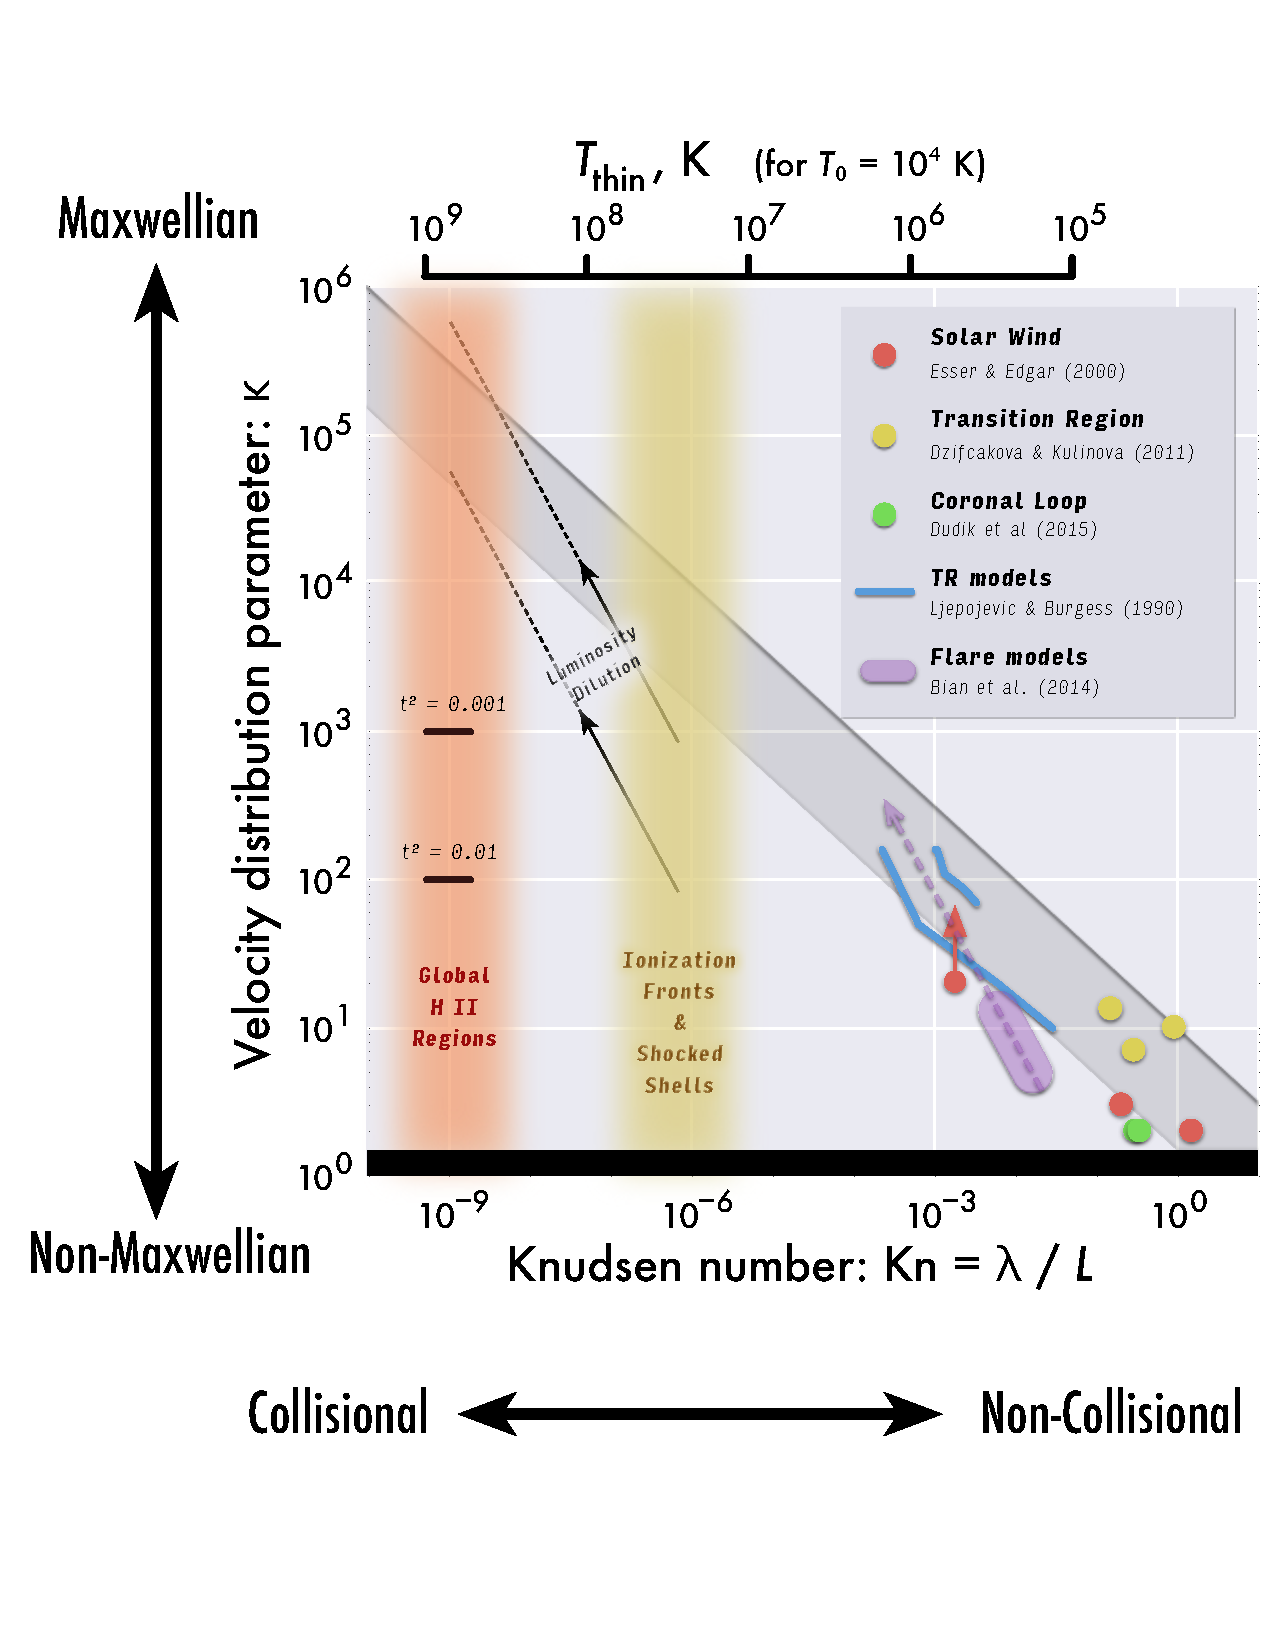
\includegraphics[width=0.8\linewidth]{kappa-versus-knudsen-graph}
  \caption{Location of \hii{} regions and selected solar phenomena in
    the plane of Kappa (non-Maxwellian parameter) versus Knudsen
    number (plasma collisionality parameter).  Colored dots show
    empirically estimated values of \(\kappa\) for the solar wind
    acceleration zone, the transition region between the chromosphere
    and corona, and for a coronal loop (see text for details).  Colored
    lines show theoretical results from modelling non-local electron transport
    downwards through the transition region, and stochastic electron
    acceleration in solar flares (again, explained in more detail in
    the text).  The diagonal darker gray band shows the relationship
    \(\kappa \sim \Kn^{-1/2}\), which has no theoretical basis but
    which roughly captures the empirical trend seen in solar
    studies. \hii{} regions and smaller-scale structures within them
    are represented by a fuzzy vertical bands to the left of the figure.
    The auxiliary horizontal scale at the top of the graph shows the
    temperature above which thermal electrons can freely stream along
    magnetic field lines over a length scale of order the size of the
    region (assuming background ionized gas at \(10^4\)\,K.)}
  \label{fig:kappa-knudsen}
\end{figure*}


\section{The collisionality of \hii{} regions and structures within
  them}
\label{sec:coll-hii-regi}

As described in the introduction, the collisionality of a plasma is
described by the Knudsen number \(\Kn = \lambda/ L\).
The relevant mean free path \(\lambda\)
is the ``deflection distance'', which is the distance over which an
electron's trajectory is deflected by 90\arcdeg{} due to very many
glancing Coulomb interactions with other charged particles
(principally electrons and protons) in the plasma.  For thermal
electrons of temperature \(T_{e}\)
and number density \(n_{e}\)this is given by
\begin{equation}
  \lambda_0 = 2.625\E{5} \frac{T_{e}^2}{n_{e} \ln\Lambda}\ \mathrm{cm}
  \label{eq:4}
\end{equation}
where the slowly varying Coulomb logarithm
(\(\ln\Lambda = 9.452 + 1.5 \ln T_{e} - 0.5 \ln n_{e} \)
for \(T_{e} < 4.2\E{5}\mathrm{\ K}\))
accounts for the cut-off in electrostatic interactions beyond the
Debye radius.  For a typical \hii{} region temperature of
\(T_{e} = 10^4 \mathrm{\ K}\)
this becomes \(\lambda_0 \simeq 1.3\E{12} n_{e}^{-1} \mathrm{\ cm}\).
This value is appropriate for electrons with velocities close to the
mean thermal velocity
\(\ubar = \sqrt{2 k T_{e}/m_{e}} \simeq 550~\kms\)
and with energies of order 1~eV.\@ The deflection mean free path is
substantially longer for higher energy electrons, scaling with
velocity as \(u^4\) or with energy as \(E^2\).  

We first estimate the Knudsen number for an idealised homogeneous
dust-free ionization-bounded \hii{} region by taking the scale length
\(L\)
as being the Strömgren radius
\(R_{s} = (3 Q_{H} / 4 \pi \alpha_{B} n^2)^{1/3}\),
where \(n \simeq n_{e}\)
is the ionized hydrogen density, \(Q_{H}\)
is the rate of ionizing photons (\(h\nu > 13.6~\U{eV}\))
emitted by the source, and
\(\alpha_{B} \simeq 2.6\E{-13}~\U{cm^3\ s^{-1}}\)
is the Case~B hydrogen recombination coefficient.  We also introduce
the global dimensionless ionization parameter
\(U = Q_{H} / 4 \pi R_{s}^2 n c\),
where \(c\)
is the speed of light, which is roughly an average ratio between the
ionizing photon density and particle density in the nebula.  We thus
find \(R_{s} = 3.46 \E{23} U n^{-1} \U{\ cm}\),
from which it follows that the Strömgren Knudsen number is
\[\Kn_{s} = 3.76\E{-12} U^{-1} ,\]
which depends only on the ionization parameter and not on the density.
It also follows from the above equations that the ionization parameter
is \(U \simeq 6\E{-4} (Q_{49} n)^{1/3}\),
where \(Q_{49}\)
is the ionizing luminosity normalized to \(10^{49}\U{\ s^{-1}}\),
which is a typical value for a single O-type star.  Values of
\(Q_{49}\), \(n\), and \(U\) for different types of ionized nebulae
are shown in Table~\ref{tab:ion-param}.  


vary from \(U \simeq 0.0006\)
for an evolved planetary nebula (\(Q_{49} \simeq 0.01\),
\(n \simeq 100\U{\ cm^{-3}}\))
up to \(U \simeq 0.02\)
for a compact \hii{} region (\(Q_{49} \simeq 1\),
\(n \simeq 10^{4}\U{\ cm^{-3}}\)),
implying \(\Kn_{s} \approx 10^{-10}\)--\(10^{-8}\).

\begin{table}
  \centering
  \caption{Physical conditions in different classes of photoionized nebulae}
  \label{tab:ion-param}
  \begin{tabular}{lllll}\hline
    Class & Example & \(Q_{49}\) & \(n\) & \(U\)\\ \hline
    OB runaway nebula & \(\zeta\)\,Oph/Sh 2-27 & 0.04 & 3 & 0.0003 \\
    Old planetary nebula & Helix Nebula & 0.01 & 100 & 0.0006 \\
    Spitzer ``Bubble'' & RCW 120 & 0.3 & 1000 & 0.004 \\
    Compact \hii{} region & Orion Nebula & 1.0 & \(10^4\) & 0.02 \\
    Giant \hii{} region & Carina, 30 Doradus &  100 & 100 & 0.02 \\ 
    Super star cluster & Arches, M82 SSCs & 1000 & \(10^6\) & 0.6 \\
    AGN Broad line regions & & & & \(\sim 0.1\) \\
    \hline
  \end{tabular}
\end{table}

Super star clusters in M82 \citep{McCrady:2007a, Krumholz:2009a}.  OB
runaway nebula \citep{Gvaramadze:2012a}.  Spitzer bubble
\citep{Deharveng:2009a}. Carina \citep{Smith:2008a} 30 Dorados \citep{Torres-Flores:2013a}

\textit{Do we want to mention case of photoevaporation flows}

\textit{Look at AGN.  BLR \citep{Baskin:2014a}, NLR
  \citep{Dopita:2002a, Groves:2004a} }

Quasar environments can have \(U > 1\)
and very hard ionizing spectra, in which case Compton heating becomes
important and the equilibrium \(T_e\)
becomes an increasing function of \(U\),
potentially reaching \(> 10^5\U{\ K}\)
\cite{Sazonov:2004a}.  \textit{We don't want to go there.}


\section{Equilibrium electron distributions in photoionized plasmas}
\label{sec:equil-electr-distr}
\newcommand\fu{\ensuremath{f_{\!u}}}
\newcommand\XXdfudt{\ensuremath{\frac{\partial \fu}{\partial t}}}
\newcommand\Xdfudt{\ensuremath{\partial \fu/\partial t}}
\newcommand\Dfudt[1]{\biggl( \XXdfudt \biggr)_{\!\scriptscriptstyle\mathrm{#1}}}
\newcommand\dfudt[1]{\ensuremath{(\Xdfudt)_{\scriptscriptstyle\mathrm{#1}}}}

In a steady state homogeneous photoionized plasma, in the absence of
external macroscopic forces, the electron velocity distribution
function \(\fu\) will satisfy the equation:
\begin{equation}
  \label{eq:1}
  \Dfudt{elastic} \!\!+\, \Dfudt{photo} \!\!+\, \Dfudt{recomb} \!\!+\, \Dfudt{inelastic} \!\!= 0, 
\end{equation}
where the four terms on the left hand side represent respectively
elastic collisions, photoionization, recombination, and inelastic
collisions.  Note that the distribution function is normalized to
\(\int_0^\infty \fu\, du = 1\).  We now consider each individual term in detail.

\newcommand\fustar{\ensuremath{\fu\smash{\!^*}}}
\paragraph{Elastic collisions} \dfudt{elastic} is the traditional
collisional redistribution integral in the Boltzmann equation
\citep[e.g.,][]{Pitaevskii:1981a}, also known as the Fokker--Planck
operator, which tends to drive the velocity distribution towards
thermal equilibrium.  A rigorous treatment of this term is difficult
and we instead adopt the BGK approximation, first introduced by
\citet{Bhatnagar:1954a}, in which the collision integral is replaced
by a simple relaxation toward a Maxwellian distribution \(\fustar\):
\begin{equation}
  \label{eq:2}
  \Dfudt{elastic} \!\!= -\frac{1}{\tau} (\fu - \fustar) ,
\end{equation}
where \(\tau = \lambda/u\) is the elastic collisional timescale. 
This is a source term (\(\dfudt{elastic} > 0\)) at velocities where
the distribution is sub-Maxwellian (\(\fu < \fu^*\)) and is a sink
term (\(\dfudt{elastic} < 0\)) at velocities where the distribution
is supra-Maxwellian (\(\fu > \fustar\)).  Thus, acting alone,
\dfudt{elastic} would drive the electrons to a Maxwellian
distribution, \(\fu \to \fustar\), on a timescale \(\tau\). 

Since the BGK approximation is only phenomenological, different
possible choices exist for the exact form of the relaxation timescale
\(\tau\)
(see \S~5.3 of \citealp{Spitzer:1956a}).  \citet{Livi:1986a} compared the
BGK approximation with evaluation of the full Fokker-Planck operator
when calculating the time-dependent relaxation of initially
anisotropic bi-Maxwellian and double-beam configurations.  They found
that the closest correspondence was obtained by using the
velocity-space friction timescale \(\tau_{F}\).  If \(\xi\)
is the electron velocity expressed in units of the mean thermal speed
(\(\xi = u /\ubar\)) then \newcommand\erf{\operatorname{erf}}
\begin{equation}
  \label{eq:3}
  \tau_{F} = \frac{\tau_0 \, \xi^2}{\erf\xi - \xi\erf'\!\xi}, 
\end{equation}
where \(\tau_0 = \lambda_0 / \ubar\), with \(\lambda_0\) given by
equation~\eqref{eq:4}, and \(\erf\), \(\erf'\) are respectively the
error function and its derivative. Other possible
choices are the slowing down timescale
\begin{equation}
  \label{eq:9}
  \tau_{s} = \xi \tau_{F} 
\end{equation}
and the deflection timescale 
\begin{equation}
  \label{eq:10}
  \tau_{d} = \frac{2 \tau_0 \, \xi^5}{(2\xi^2 - 1)\erf\xi + \xi\erf'\!\xi} .  
\end{equation}
All three are shown in Figure~\ref{fig:relax}, where it is apparent
that only \(\tau_F\)
diverges both for very small and very large velocities, meaning that
elastic collisions take longer to Maxwellianize the low-energy and
high-energy tails of the distribution.  The other two timescales
increase monotonically with \(u\),
meaning that the low velocity electrons will Maxwellianize most
rapidly.  Below, we investigate the effects of using each of these
timescales in the relaxation operator.

\newcommand*{\vcenteredhbox}[1]{\begingroup
  \setbox0=\hbox{#1}\parbox{\wd0}{\box0}\endgroup}
\begin{figure}
  \vcenteredhbox{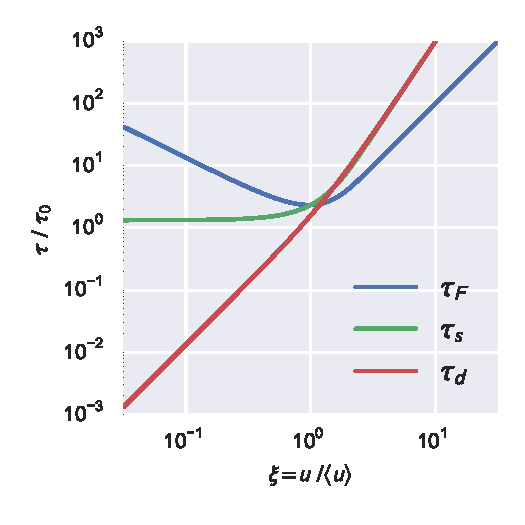
\includegraphics[width=0.45\linewidth]{relax_timescales}}
  \vcenteredhbox{%
    \begin{tabular}{lll}\hline
      & \(u \ll \ubar\) & \(u \gg \ubar\) \\ \hline
      \(\tau_F\) & \(\propto u^{-1} \) & \(\propto u^{2} \) \\
      \(\tau_s\) & constant & \(\propto u^{3} \) \\
      \(\tau_d\) & \(\propto u^{2} \) & \(\propto u^{3} \) \\ \hline
    \end{tabular}}
  \caption{Three different candidate relaxation timescales as a
    function of electron velocity in thermal units. Velocity-space
    friction timescale \(\tau_F\)
    (blue line), slowing down time \(\tau_s\)
    (green line), and deflection time \(\tau_d\)
    (red line).  Asymptotic behaviors for small and large velocities
    are shown in the table.}
  \label{fig:relax}
\end{figure}

\paragraph{Photoionizations} \dfudt{photo} represents the rate of
production of photo-electrons with velocity \(u\) due to the
photoionization of neutral hydrogen or atoms/ions of other elements.
Consider the photoionization of H from the ground level (see \S~2.2 of
\citealp{2006agna.book.....O}) by photons of energy \(h\nu\).
The resultant photo-electron will have energy \(\frac12 m_e u^2 = h\nu
- h\nu_0\), where \(h\nu_0 = 13.6~\U{eV}\) is the H ionization
potential.  
\begin{figure}[tp]
  \centering
  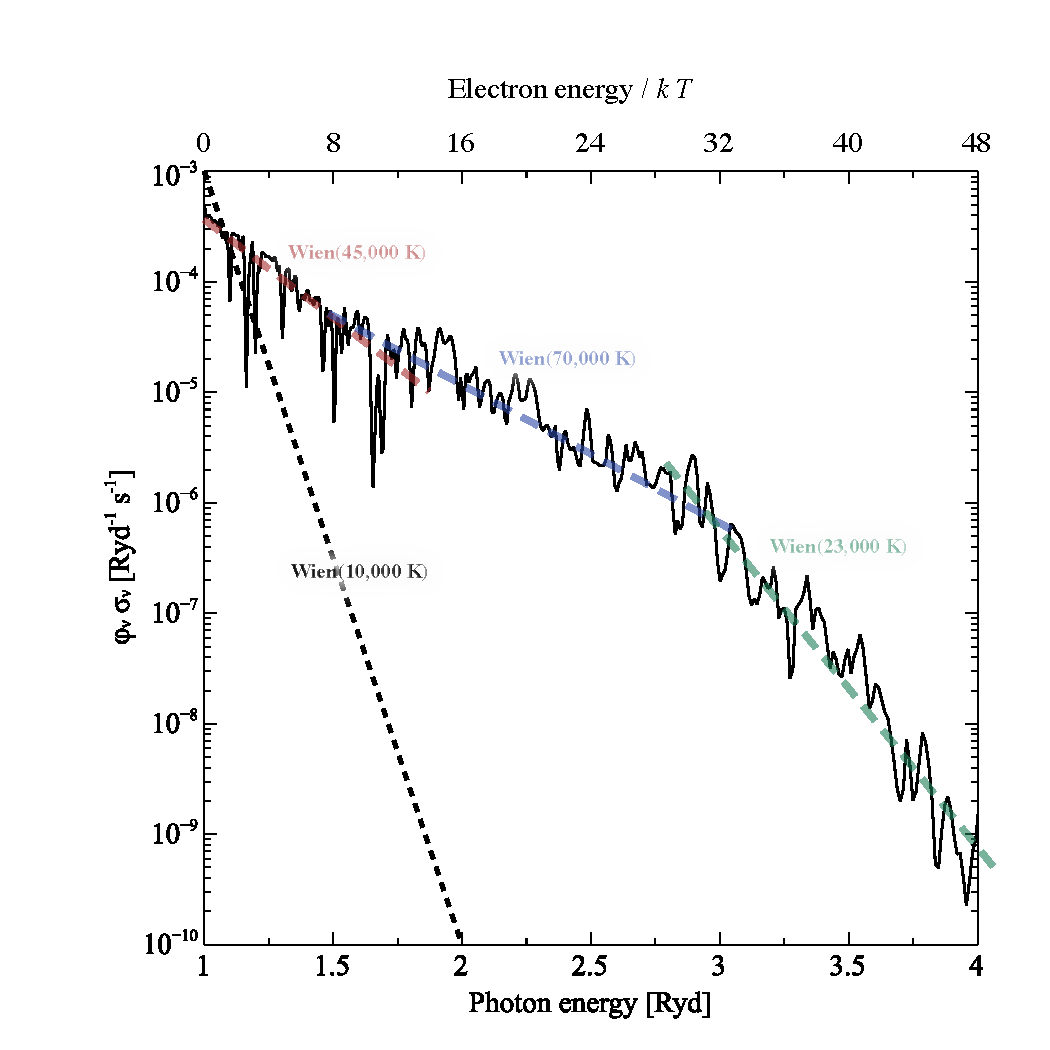
\includegraphics[width=0.9\linewidth]{edited-photoelectron-yield-orion}
  \caption{Semilogarithmic plot of photoelectric yield as a function
    of ionizing photon energy (lower horizontal scale) or
    photoelectron energy (upper horizontal scale) from a Cloudy model
    of the Orion Nebula.  Dashed colored lines show approximate
    piecewise Wien (exponential) fits to the data.  Dashed black line
    shows high energy tail of 10,000~K Maxwellian distribution.}
  \label{fig:photoelec}
\end{figure}%
The ionizing photon intensity is represented by 
\begin{equation}
  \label{eq:8}
  \phi_\nu = \frac{4\pi J_\nu}{h\nu} \ \U{photons\ s^{-1}\ cm^{-2} \ Hz^{-1}}, 
\end{equation}
where \(J_\nu\)
is the mean intensity of the radiation field.  If \(n(\mathrm{H^0})\)
is the number density of neutral H, and \( a_\nu \)
is the frequency-dependent photoionization cross-section
(approximately proportional to \(\nu^{-3}\)
for \(\nu > \nu_0\)),
then the photo-electron production rate per unit volume and per unit
velocity interval is
\begin{equation}
  \label{eq:6}
  n_e \Dfudt{photo} \!\! = n(\mathrm{H^0})  \phi_\nu a_\nu \frac{d\nu}{d u} . 
\end{equation}
Similar contributions will arise from the ionization of neutral
helium, singly ionized helium, and heavier elements.
Figure~\ref{fig:photoelec} shows the product \(\phi_\nu a_\nu\)
(except in energy rather than frequency units) at the illuminated face
of a Cloudy model of the Orion Nebula, with the ionizing spectrum
calculated from stellar atmosphere models \citep{2003ApJS..146..417L}
of the 5 OB stars of the Trapezium cluster \citep{Ferland:2012a}.
\emph{Does this include dust photoionization?  Does it include the OTS
diffuse field?}.  The photoelectric
yield can be approximately fit by piecewise exponential Wien
functions, \(\exp(-E/k T_*)\),
as shown on the figure.  For photon energies between the H\(^0\)
and He\(^0\)
ionization edges (1 to 1.8 Rydbergs, corresponding to photoelectron
energies \(\lesssim 10 k T_e\)),
we find \(T_* \simeq 45,000\)~K\@.
This is close to the effective temperature of the most luminous
ionizing star, and much larger than the equilibrium electron
temperature in the \hii{} region, meaning that the high-energy tail of
\(\fu\) will be preferentially populated by this mechanism.

\paragraph{Recombinations} \dfudt{recomb} represents the rate of loss
of electrons due to radiative recombination with protons and other
ions.  For recombinations to all excited (\(n > 1\))
bound states \(nL\)
of hydrogen, the electron loss rate per unit volume and unit velocity
interval is (e.g., \S~4.3 of \citealp{Ferland:2012a})
\begin{equation}
  \label{eq:11}
  n_e \Dfudt{recomb} = -n_e n_p u \fu \sum_{n=2}^\infty \sum_{L=0}^{n-1} \sigma(\mathrm{H}^0_{nL},\, u),  
\end{equation}
where \(\sigma(\mathrm{H}^0_{nL},\, u)\) are the radiative recombination
cross-sections, which can be expressed in terms of the photoionization
cross-sections as 
\begin{equation}
  \label{eq:5}
  \sigma(\mathrm{H}^0_{nL},\, u) = (2 L + 1) \frac{h^2 \nu^2}{m_e^2 c^2 u^2} \, a_\nu(\mathrm{H}^0_{nL})
\end{equation}
in which \(h\nu = \frac12 m_e u^2 + h\nu_0/n^2\). 
\textit{Do we just ignore the recombinations to the ground state?
  Does Cloudy have a way of simply printing out these terms.  We could
  perhaps calculate them from the free-bound continuum spectra.}

\paragraph{Inelastic collisions} \dfudt{inelastic} represents both a
source of lower velocity electrons and also a sink of higher velocity
electrons due to the collisional excitation of bound-bound transitions
in atoms and ions, followed by their spontaneous radiative decay.  It
is only important for transitions with critical densities
\(n_{\mathrm{crit}} \gtrsim n_e\)
since super-elastic collisional de-excitations are in equilibrium with
inelastic collisional excitations in the limit
\(n_{\mathrm{crit}} \ll n_e\),
leading to zero net contribution to \dfudt{inelastic}.  As an example,
we consider the \({}^3P\)--\({}^1D_2\)
transition in \oiii{}, which gives emission of the \Wav{5007} and
\Wav{4959} optical lines.

\textit{Insert material gleaned from \citet{Storey:2014a}.  Their
  Fig~1(c) gives the energy-resolved collision strength, but it only
  goes up to 0.05 Rydbergs, which is less than \(kT \).
}

Electrons with energies greater than 0.75~Rydberg (\(\xi \gtrsim
3.5\)) can collisionally excite the H\(^0\) Lyman lines.  At nebular
temperatures this is not an important cooling mechanism because the
Maxwellian population of such high energy electrons is so small: \(\fu
\sim e^{-\xi^2} \approx 10^{-5}\).  However, for the few electrons that
\emph{do} have such high energies it will be an important sink term.
Similarly, electrons more energetic than 1~Rydberg can collisionally
ionize H\(^0\), which can also be considered as a kind of inelastic
collision in which a high energy electron is converted into two lower
energy electrons with velocities \(u'\) and \(u''\) that satisfy 
\begin{equation}
  \label{eq:12}
  \frac12 m_e u^2 = h\nu_0 + \frac12 m_e u'^2 + \frac12 m_e u''^2 .
\end{equation}
 



\section{Diffusion of high energy electrons through photoionized gas}
\label{sec:diff-high-energy}


\subsection{Cooling zone behind low-velocity shocks}
\label{sec:cooling-zone-behind}

Spitzer--Härm approximation is valid for \(\xi < \xi_c =
\Kn_{T}^{-1/4}\) \citep{Shoub:1983a}, where the temperature-gradient Knudsen number is
\(\Kn_T = \lambda_0 d\ln T/ d z\). So, with \(\Kn = 0.0065\) which I
get from the shock models, we find \(\xi_c = 3.5\). Thus, for \(\xi <
3.5\) we have 
\begin{equation}
  \label{eq:7}
  \fu(\xi, \mu, z) = \fu^*(\xi, z) \biggl[ 
  1 + \mu\, \Kn\, D(\xi) + O(\Kn^2)
  \biggr]
\end{equation}
where \(D(\xi)\) is given in Table~II of \citet{Spitzer:1953a}.  This
implies that the deviation of the angle-averaged distribution function
from  Maxwellian is of order \((\Kn)^2\) for \(\xi < \xi_c\).

\textit{We should check this against results of BGK calculations. }


\subsection{Leakage of hot electrons from stellar wind bubbles}
\label{sec:diff-hot-electr}

Recent models of stellar wind bubbles inside \hii{} regions \citep{Mackey:2015a}

Survey of \hii{} regions in LMC and SMC \citep{Lopez:2014a} give X-ray
emitting hot gas with \(T = 2\)--\(8\E{6}\U{\ K}\) and density
\(0.01\)--\(0.3\ \pcc\). \textit{Also look at \dots } Carina \citep{Townsley:2011b}

Need to consider inelastic interactions that would effect the hot
electrons, such as collisional ionization.  But according to \S11.3.3
of \citet{2006agna.book.....O} this is only important for ionization
fractions less than 0.9 (should it be 0.1?).  This is treated in more detail in
\citet{Furlanetto:2010a} who carry out Monte Carlo simulations of
electrons from 10~eV to 10~keV, albeit for primordial abundances,
finding that heating is completely dominant when the gas is more than
a little bit ionized.  For instance, with ionization fraction of
0.9--0.999 and 3~keV electrons, 98\% of energy goes into heating
through elastic collisions and 2\% goes into ionization, nearly all of
which is of He.  

\textit{They have an interesting way of treating the energy loss in
  the elastic collisions by discretization.  Assume an arbitrary fixed
  fraction \(f\)
  of energy is lost in individual ``collision'' events, for which one
  can work out an effective cross-section, which will be
  \(\propto 1/f\).
  They cite \citet{Habing:1979a} and \citet{Shull:1979a} for this.
  Perhaps we could adapt it to our case, but we need to take a quite
  small \(f \sim 10^{-4}\)
  so that the energy given to the thermal electrons in each
  ``interaction'' is a fraction of an eV. }

\textit{In \citet{Spitzer:1969a} it is argued that the dispersion in
  energies of initially monoenergetic non-thermal electrons is small as they
  lose energy by elastic collisions.  The quote is  
  \begin{quotation}
    Hence, if a group of secondary electrons all have the same energy
    initially, their dispersion of energies after one energy-loss time
    will be small compared with their initial energy.  
  \end{quotation}
  It seems that the energy loss of the non-thermal electrons does not
  occur via a ``cascade'' as I had originally supposed, but rather is
  a gradual slowing down of the high-velocity electron, with the
  energy going in to general heating of the thermal electrons.  If
  this is true, then it makes the BGK approximation much more
  defensible, even for this case.
}

Also include Auger electrons from inner shell photoionization by
X-rays as a source of high energy electrons.  Compared with those that
come from stellar wind bubble these have the advantage that they are
created throughout the nebula. 

\textit{Dust contribution from \citet{Weingartner:2006a}}

\subsection{Effects of magnetic fields}
\label{sec:effects-magn-fields}

Diffusion across field lines is greatly suppressed.  \emph{But look
  into Bohm diffusion (only 2D case?) and Hsu diffusion (3D), which
  give perpendicular transport coefficients much larger than the
  classical values.}

\clearpage

\bibliography{BibdeskLibrary-slavoj}



\end{document}

%%% Local Variables:
%%% mode: latex
%%% TeX-master: t
%%% End:
